% This file was converted to LaTeX by Writer2LaTeX ver. 1.0.2
% see http://writer2latex.sourceforge.net for more info
\documentclass[twoside,letterpaper]{article}
\usepackage[latin1]{inputenc}
\usepackage[T1]{fontenc}
\usepackage[english]{babel}
\usepackage{amsmath}
\usepackage{amssymb,amsfonts,textcomp}
\usepackage{color}
\usepackage{array}
\usepackage{supertabular}
\usepackage{hhline}
\usepackage{hyperref}
\usepackage{cite}
\usepackage{etoolbox}
\usepackage{textcomp}
\usepackage{textgreek}
\patchcmd{\thebibliography}{\section*{\refname}}{}{}{}
\hypersetup{pdftex, colorlinks=true, linkcolor=blue, citecolor=blue, filecolor=blue, urlcolor=blue, pdftitle=SYSTEMS AND SOFTWARE REQUIREMENTS SPECIFICATION (SSRS) TEMPLATE, pdfauthor=Clinton Jeffery, pdfsubject=, pdfkeywords=}
\usepackage[pdftex]{graphicx}
% Outline numbering
\setcounter{secnumdepth}{5}
\renewcommand\thesection{\arabic{section}}
\renewcommand\thesubsection{\arabic{section}.\arabic{subsection}}
\renewcommand\thesubsubsection{\arabic{section}.\arabic{subsection}.\arabic{subsubsection}}
\renewcommand\theparagraph{\arabic{section}.\arabic{subsection}.\arabic{subsubsection}.\arabic{paragraph}}
\renewcommand\thesubparagraph{\arabic{section}.\arabic{subsection}.\arabic{subsubsection}.\arabic{paragraph}.\arabic{subparagraph}}
\makeatletter
\newcommand\arraybslash{\let\\\@arraycr}
\makeatother
% Page layout (geometry)
\setlength\voffset{-1in}
\setlength\hoffset{-1in}
\setlength\topmargin{0.5in}
\setlength\oddsidemargin{1in}
\setlength\evensidemargin{1in}
\setlength\textheight{8.278in}
\setlength\textwidth{6.5in}
\setlength\footskip{0.561in}
\setlength\headheight{0.5in}
\setlength\headsep{0.461in}
% Footnote rule
\setlength{\skip\footins}{0.0469in}
\renewcommand\footnoterule{\vspace*{-0.0071in}\setlength\leftskip{0pt}\setlength\rightskip{0pt plus 1fil}\noindent\textcolor{black}{\rule{0.25\columnwidth}{0.0071in}}\vspace*{0.0398in}}
% Pages styles
\makeatletter
\newcommand\ps@Standard{
  \renewcommand\@oddhead{\selectlanguage{english}\rmfamily\color{black} College Of Engineering, Trivandrum\hfill \hfill Project Design}
  \renewcommand\@evenhead{\@oddhead}
  \renewcommand\@oddfoot{\foreignlanguage{english}{\textcolor{black}{SRS Page }}\foreignlanguage{english}{\textcolor{black}{\thepage{}}}}
  \renewcommand\@evenfoot{\@oddfoot}
  \renewcommand\thepage{\arabic{page}}
}
\newcommand\ps@Convertviii{
  \renewcommand\@oddhead{}
  \renewcommand\@evenhead{\@oddhead}
  \renewcommand\@oddfoot{}
  \renewcommand\@evenfoot{\@oddfoot}
  \renewcommand\thepage{\arabic{page}}
}
\newcommand\ps@Convertvii{
  \renewcommand\@oddhead{}
  \renewcommand\@evenhead{\@oddhead}
  \renewcommand\@oddfoot{}
  \renewcommand\@evenfoot{\@oddfoot}
  \renewcommand\thepage{\arabic{page}}
}
\newcommand\ps@Convertvi{
  \renewcommand\@oddhead{}
  \renewcommand\@evenhead{\@oddhead}
  \renewcommand\@oddfoot{}
  \renewcommand\@evenfoot{\@oddfoot}
  \renewcommand\thepage{\arabic{page}}
}
\newcommand\ps@Convertv{
  \renewcommand\@oddhead{}
  \renewcommand\@evenhead{\@oddhead}
  \renewcommand\@oddfoot{}
  \renewcommand\@evenfoot{\@oddfoot}
  \renewcommand\thepage{\arabic{page}}
}
\newcommand\ps@Convertiv{
  \renewcommand\@oddhead{}
  \renewcommand\@evenhead{\@oddhead}
  \renewcommand\@oddfoot{}
  \renewcommand\@evenfoot{\@oddfoot}
  \renewcommand\thepage{\arabic{page}}
}
\newcommand\ps@Convertii{
  \renewcommand\@oddhead{}
  \renewcommand\@evenhead{\@oddhead}
  \renewcommand\@oddfoot{}
  \renewcommand\@evenfoot{\@oddfoot}
  \renewcommand\thepage{\arabic{page}}
}
\newcommand\ps@FirstPage{
  \renewcommand\@oddhead{}
  \renewcommand\@evenhead{\@oddhead}
  \renewcommand\@oddfoot{}
  \renewcommand\@evenfoot{\@oddfoot}
  \renewcommand\thepage{\arabic{page}}
}
\makeatother
\pagestyle{Standard}
\setlength\tabcolsep{1mm}
\renewcommand\arraystretch{1.3}
% footnotes configuration
\makeatletter
\renewcommand\thefootnote{\arabic{footnote}}
\makeatother
\title{SOFTWARE REQUIREMENT SPECIFICATION}
\author{Kevin Joseph, Jayadeep K M, Mohammed. Nisham}
\date{\today}
\begin{document}

\clearpage{\centering\selectlanguage{english}\bfseries\color{black}
Design Document FOR 
\par}


\bigskip

{\centering\selectlanguage{english}\bfseries\color{black}
Decision making using Reinforced Deep Learning
\par}


\bigskip

\centering

\includegraphics[width=3cm]{images/logo.jpg}

\bigskip

{\centering\selectlanguage{english}\bfseries\color{black}
\today
\par}


\bigskip


\bigskip

{\centering\selectlanguage{english}\bfseries\color{black}
Prepared for:
\par}

{\centering\selectlanguage{english}\color{black}
Btech Project Interim Evaluation
\par}


\bigskip


\bigskip

{\centering\selectlanguage{english}\bfseries\color{black}
Prepared by:
\par}

{\centering\selectlanguage{english}\color{black}
Kevin Joseph, Jayadeep K.M. , Mohd. Nisham
\par}
\bigskip
{\centering\selectlanguage{english}\bfseries\color{black}
Guide:
\par}

{\centering\selectlanguage{english}\color{black}
Vipin Vasu\\
vipin@cet.ac.in\\
\par}
\bigskip
{\centering\selectlanguage{english}\bfseries\color{black}
College Of Engineering, Trivandrum
\par}

\clearpage{\centering\selectlanguage{english}\bfseries\color{black}
\par}

{\centering\selectlanguage{english}\bfseries\color{black}
TABLE OF CONTENTS
\par}


\bigskip

{\selectlanguage{english}\bfseries\color{black}
Section\ \ Page}

\setcounter{tocdepth}{9}
\renewcommand\contentsname{}
\tableofcontents

\bigskip

\clearpage\clearpage\setcounter{page}{1}\pagestyle{Convertii}
\section[Background and Literature]
{\selectlanguage{english}\rmfamily\bfseries\color{black}
Background and Literature}

\subsection[Reinforcement Learning]{\selectlanguage{english}\rmfamily\bfseries\color{black}
Reinforcement Learning}
{\selectlanguage{english}\color{black}
Consider the game Breakout. In this game you control a paddle at the bottom of the screen and have to bounce the ball back to clear all the bricks in the upper half of the screen. Each time you hit a brick, it disappears and your score increases you get a reward.\\

\centering
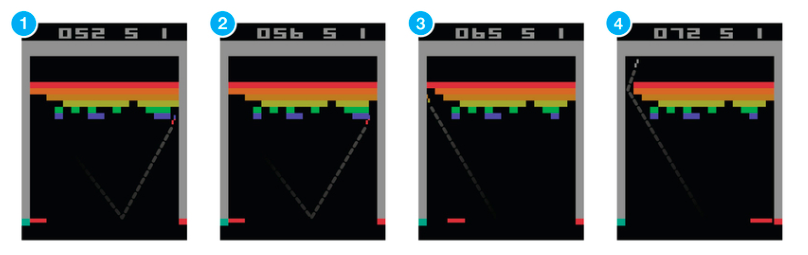
\includegraphics[width=10cm]{images/breakout.png}\\
Suppose you want to teach a neural network to play this game. Input to your network would be screen images, and output would be three actions left, right or fire to launch the ball. It would make sense to treat it as a classification problem for each game screen you have to decide, whether you should move left, right or press fire. Sounds straightforward, Sure, but then you need training examples, and a lots of them. Of course you could go and record game sessions using expert players, but thats not really how we learn. We dont need somebody to tell us a million times which move to choose at each screen. We just need occasional feedback that we did the right thing and can then figure out everything else ourselves.\\
\bigskip
This is the task reinforcement learning tries to solve. Reinforcement learning lies somewhere in between supervised and unsupervised learning. Whereas in supervised learning one has a target label for each training example and in unsupervised learning one has no labels at all, in reinforcement learning one has sparse and time-delayed labels  the rewards. Based only on those rewards the agent has to learn to behave in the environment.\\
\bigskip
While the idea is quite intuitive, in practice there are numerous challenges. For example when you hit a brick and score a reward in the Breakout game, it often has nothing to do with the actions (paddle movements) you did just before getting the reward. All the hard work was already done, when you positioned the paddle correctly and bounced the ball back. This is called the credit assignment problem i.e., which of the preceding actions was responsible for getting the reward and to what extent.\\
\bigskip
Once you have figured out a strategy to collect a certain number of rewards, should you stick with it or experiment with something that could result in even bigger rewards? In the above Breakout game a simple strategy is to move to the left edge and wait there. When launched, the ball tends to fly left more often than right and you will easily score about 10 points before you die. Will you be satisfied with this or do you want more? This is called the explore-exploit dilemma should you exploit the known working strategy or explore other, possibly better strategies.\\
\bigskip
Reinforcement learning is an important model of how we (and all animals in general) learn. Praise from our parents, grades in school, salary at work these are all examples of rewards. Credit assignment problems and exploration exploitation dilemmas come up every day both in business and in relationships. Thats why it is important to study this problem, and games form a wonderful sandbox for trying out new approaches.}

\subsection[Markov Decision Process]{\selectlanguage{english}\rmfamily\bfseries\color{black}
Markov Decision Process}
{\selectlanguage{english}\color{black}
Suppose you are an agent, situated in an environment (e.g. Breakout game). The environment is in a certain state (e.g. location of the paddle, location and direction of the ball, existence of every brick and so on). The agent can perform certain actions in the environment (e.g. move the paddle to the left or to the right). These actions sometimes result in a reward (e.g. increase in score). Actions transform the environment and lead to a new state, where the agent can perform another action, and so on. The rules for how you choose those actions are called policy. The environment in general is stochastic, which means the next state may be somewhat random (e.g. when you lose a ball and launch a new one, it goes towards a random direction).\\

\centering
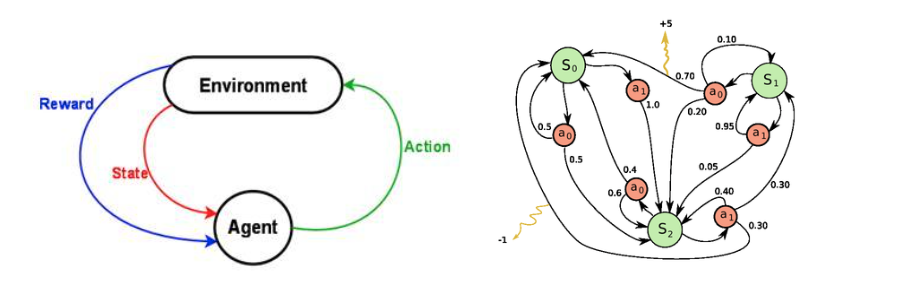
\includegraphics[width=10cm]{images/mdp.png}\\
The set of states and actions, together with rules for transitioning from one state to another, make up a Markov decision process. One episode of this process (e.g. one game) forms a finite sequence of states, actions and rewards:\\
\centering
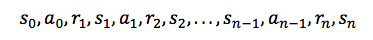
\includegraphics[width=10cm]{images/mdp2.png}\\
Here si represents the state, ai is the action and ri+1 is the reward after performing the action. The episode ends with terminal state sn (e.g. game over screen). A Markov decision process relies on the Markov assumption, that the probability of the next state si+1 depends only on current state si and action ai, but not on preceding states or actions.
}

\subsection[Discounted Future Reward]{\selectlanguage{english}\rmfamily\bfseries\color{black}
Discounted Future Reward}

{\selectlanguage{english}\color{black}
To perform well in the long-term, we need to take into account not only the immediate rewards, but also the future rewards we are going to get. How should we go about that?\\

Given one run of the Markov decision process, we can easily calculate the total reward for one episode:\\
\centering
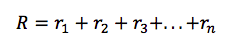
\includegraphics[width=5cm]{images/dfr.png}\\
Given that, the total future reward from time point t onward can be expressed as:\\
\centering
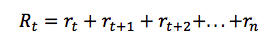
\includegraphics[width=7cm]{images/dfr2.png}\\
But because our environment is stochastic, we can never be sure, if we will get the same rewards the next time we perform the same actions. The more into the future we go, the more it may diverge. For that reason it is common to use discounted future reward instead:\\
\centering
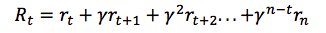
\includegraphics[width=9cm]{images/dfr3.png}\\
Here Y is the discount factor between 0 and 1 the more into the future the reward is, the less we take it into consideration. It is easy to see, that discounted future reward at time step t can be expressed in terms of the same thing at time step t+1:\\
\centering
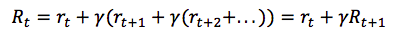
\includegraphics[width=10cm]{images/dfr4.png}\\
If we set the discount factor Y=0, then our strategy will be short sighted and we rely only on the immediate rewards. If we want to balance between immediate and future rewards, we should set discount factor to something like Y=0.9. If our environment is deterministic and the same actions always result in same rewards, then we can set discount factor Y=1.\\

A good strategy for an agent would be to always choose an action that maximizes the (discounted) future reward.
}

\subsection[Q-Learning]{\selectlanguage{english}\rmfamily\bfseries\color{black}
Q-Learning}
{\selectlanguage{english}\color{black}
In Q-learning we define a function Q(s, a) representing the maximum discounted future reward when we perform action a in state s, and continue optimally from that point on.\\
\centering
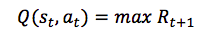
\includegraphics[width=5cm]{images/q.png}\\
The way to think about Q(s, a) is that it is the best possible score at the end of the game after performing action a in state s. It is called Qfunction, because it represents the quality of a certain action in a given state.\\

This may sound like quite a puzzling definition. How can we estimate the score at the end of game, if we know just the current state and action, and not the actions and rewards coming after that? We really cant. But as a theoretical construct we can assume existence of such a function. Just close your eyes and repeat to yourself five times: Q(s, a) exists, Q(s, a) exists, . Feel it?\\

If youre still not convinced, then consider what the implications of having such a function would be. Suppose you are in state and pondering whether you should take action a or b. You want to select the action that results in the highest score at the end of game. Once you have the magical Q-function, the answer becomes really simple pick the action with the highest Q value!\\
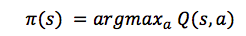
\includegraphics[width=5cm]{images/q2.png}\\
\centering
The above policy, the rule how we choose an action in each state.\\

OK, how do we get that Q function then? Lets focus on just one transition <s, a, r, s\textquotesingle>. Just like with discounted future rewards in the previous section, we can express the Q value of state s and action a in terms of the Q value of the next state s\textquotesingle.\\
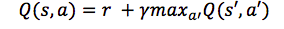
\includegraphics[width=5cm]{images/q3.png}\\
This is called the Bellman equation. If you think about it, it is quite logical maximum future reward for this state and action is the immediate reward plus maximum future reward for the next state.

The main idea in Q-learning is that we can iteratively approximate the Q-function using the Bellman equation. In the simplest case the Q-function is implemented as a table, with states as rows and actions as columns. The gist of the Q learning algorithm is as simple as the following:
\centering
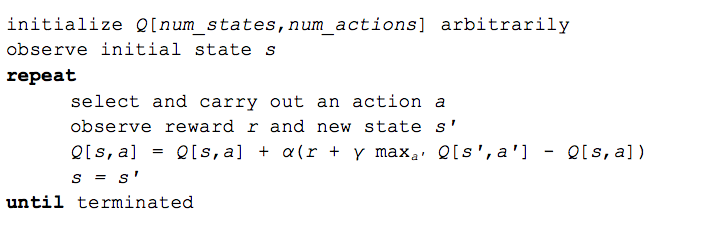
\includegraphics[width=10cm]{images/q4.png}\\

}
\bigskip
\clearpage\section[Design]{\selectlanguage{english}\rmfamily\bfseries\color{black}
Design}
\subsection[Deep Q Network]{\selectlanguage{english}\rmfamily\bfseries\color{black}
Deep Q Network}


{\selectlanguage{english}\color{black}
The state of the environment in the Breakout game can be defined by the location of the paddle, location and direction of the ball and the presence or absence of each individual brick. This intuitive representation however is game specific. Could we come up with something more universal, that would be suitable for all the games? The obvious choice is screen pixels they implicitly contain all of the relevant information about the game situation, except for the speed and direction of the ball. Two consecutive screens would have these covered as well.\\

If we apply the same preprocessing to game screens as in the DeepMind paper, take the four last screen images, resize them to 84x84 and convert to grayscale with 256 gray levels. This means 10\textsuperscript{67970} rows in our imaginary Q table, more than the number of atoms in the known universe! One could argue that many pixel combinations (and therefore states) never occur we could possibly represent it as a sparse table containing only visited states. Even so, most of the states are very rarely visited and it would take a lifetime of the universe for the Q table to converge. Ideally, we would also like to have a good guess for Q values for states we have never seen before.\\

This is the point where deep learning steps in. Neural networks are exceptionally good at coming up with good features for highly structured data. We could represent our Q function with a neural network, that takes the state (four game screens) and action as input and outputs the corresponding Q value. Alternatively we could take only game screens as input and output the Q-value for each possible action. This approach has the advantage, that if we want to perform a Q value update or pick the action with the highest Q value, we only have to do one forward pass through the network and have all Q values for all actions available immediately.\\
\centering
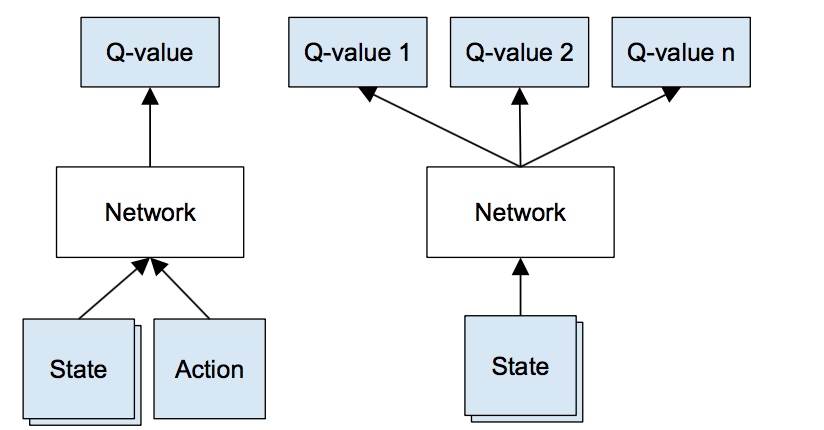
\includegraphics[width=10cm]{images/deep.png}\\
\bigskip
\centering
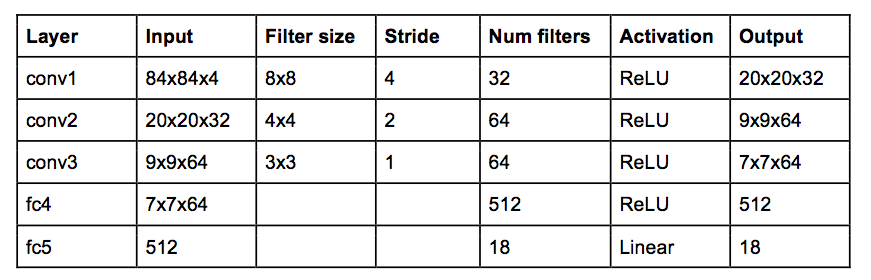
\includegraphics[width=10cm]{images/deep2.png}\\
}

\subsection[Exploration Exploitation]{\selectlanguage{english}\rmfamily\bfseries\color{black}
Exploration Exploitation}
{\selectlanguage{english}\color{black}
Q-learning attempts to solve the credit assignment problem it propagates rewards back in time, until it reaches the crucial decision point which was the actual cause for the obtained reward. But we havent touched the exploration exploitation dilemma yet\\
\bigskip
Firstly observe, that when a Q-table or Q-network is initialized randomly, then its predictions are initially random as well. If we pick an action with the highest Q-value, the action will be random and the agent performs crude exploration. As a Q-function converges, it returns more consistent Q-values and the amount of exploration decreases. So one could say, that Q-learning incorporates the exploration as part of the algorithm. But this exploration is greedy, it settles with the first effective strategy it finds.\\
\bigskip
A simple and effective fix for the above problem is \textepsilon greedy exploration with probability \textepsilon choose a random action, otherwise go with the greedy action with the highest Q-value. In their system DeepMind actually decreases \textepsilon over time from 1 to 0.1 in the beginning the system makes completely random moves to explore the state space maximally, and then it settles down to a fixed exploration rate.\\
}

\subsection[Deep Q-Algorithm]{\selectlanguage{english}\rmfamily\bfseries\color{black}
Deep Q-Algorithm}

{\selectlanguage{english}\color{black}
\centering
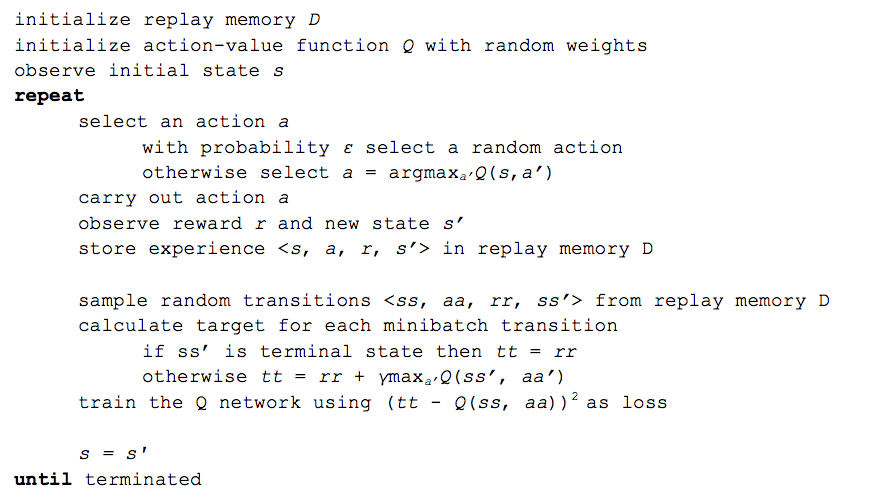
\includegraphics[width=10cm]{images/deep3.png}\\}

\clearpage\setcounter{page}{1}\pagestyle{Convertv}
\subsection[Class Diagram]{\selectlanguage{english}\rmfamily\bfseries\color{black}
Class Diagram}
{\selectlanguage{english}\color{black}
\centering
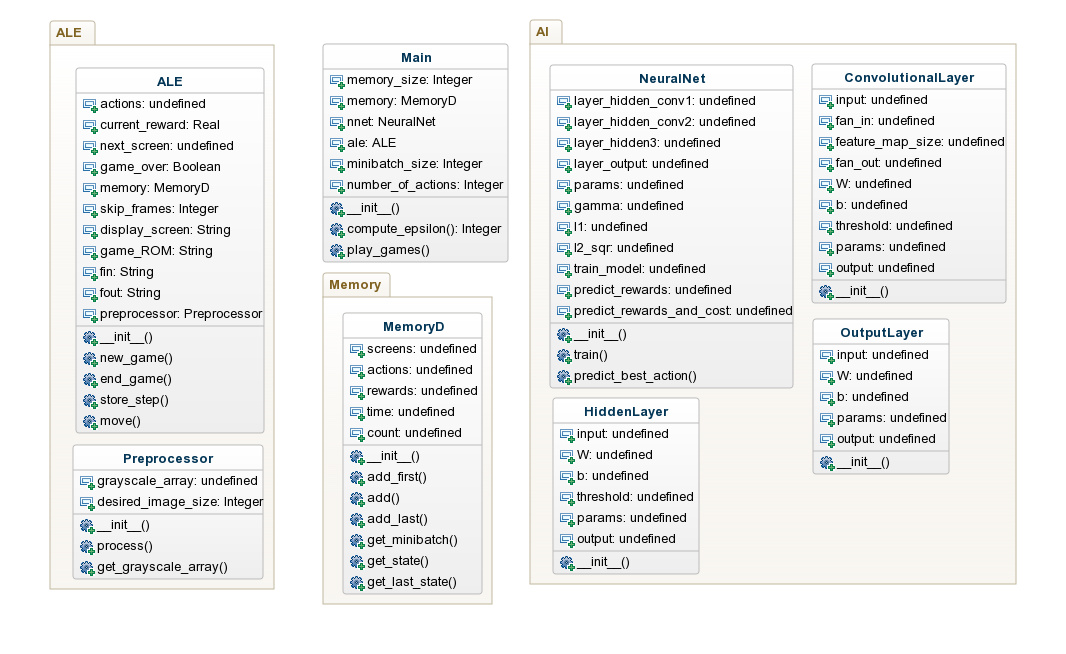
\includegraphics[width=15cm]{images/jpeg.jpg}\\
}
\end{document}
